%----------------------------------------------------------------------------------------
%	PACKAGES & THEMES
%----------------------------------------------------------------------------------------

\documentclass[8pt]{beamer}

\usepackage{etex}
\mode<presentation> {
\usetheme{Vilanova}
}

\usepackage[french]{babel}
\usepackage[utf8]{inputenc}
\usepackage{array}
\usepackage{graphicx}
\usepackage{booktabs}
\usepackage{amsmath,amssymb,amsthm}
\usepackage{xcolor}
\usepackage{tikz}
\usetikzlibrary{arrows}
\usepackage{pifont}
\usepackage{listings,color}

\definecolor{listcomment}{rgb}{0.0,0.5,0.0}
\definecolor{listkeyword}{rgb}{0.0,0.0,0.5}
\definecolor{listnumbers}{gray}{0.65}
\definecolor{listlightgray}{gray}{0.955}
\definecolor{listwhite}{gray}{1.0}

\AtBeginSection[]
{
\addtocounter{framenumber}{-1}
\begin{frame}
\frametitle{Sommaire}
\tableofcontents[currentsection]
\end{frame}}

%----------------------------------------------------------------------------------------
%	PAGE TITRE
%----------------------------------------------------------------------------------------
\title{Orfeo ToolBox}
\subtitle{Un logiciel libre pour le traitement d'images de télédétection (màj.  pour 5.4)}
\author{Equipe OTB CNES}% date and event here
\date{}

\pgfdeclareimage[height=96mm,width=128mm]{background}{images/fondsClairSansLogo}
\pgfdeclareimage[height=0.2cm]{cc}{images/CC-licence.png}
\setbeamertemplate{background}{\pgfuseimage{background}}
\pgfdeclareimage[height=0.6cm]{logoIncrust}{images/logoIncrust}
\pgfdeclareimage[height=0.6cm]{logo_cnes}{images/logo_cnes}
\logo{
\begin{tabular}{p{0.22\textwidth}p{0.58\textwidth}p{0.1\textwidth}p{0.1\textwidth}}
\href{http://www.cnes.fr}{\pgfuseimage{logo_cnes}}
& \vspace{-0.03\textwidth} \scriptsize{} % date and event here
& \href{http://creativecommons.org/licenses/by-sa/3.0/}{\pgfuseimage{cc}} & \href{http://www.orfeo-toolbox.org}{\pgfuseimage{logoIncrust}}\\
\end{tabular}
}

\titlegraphic{\vspace*{-5em}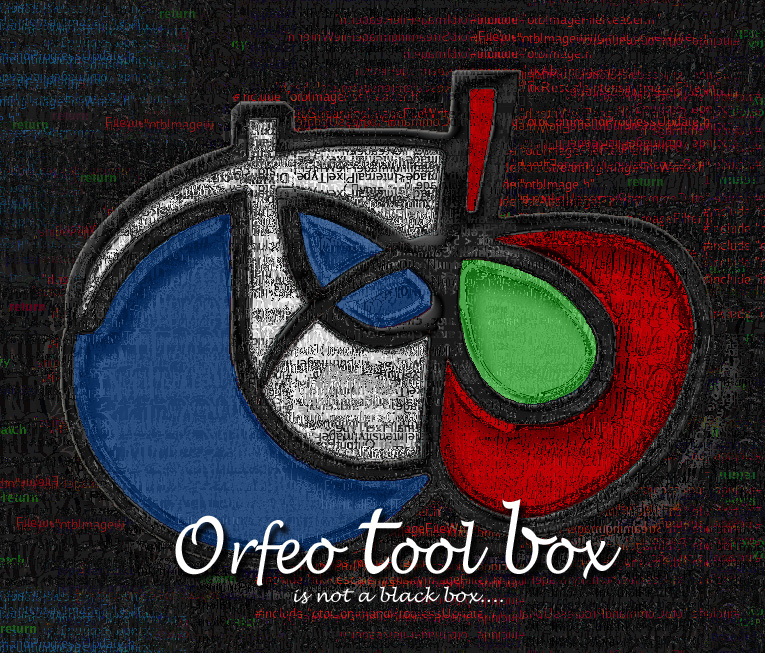
\includegraphics[width=.5\textwidth]{images/LOGOTB_blackbox.png}}

\begin{document}
\begin{frame}
\titlepage
\end{frame}

\section*{Introduction}

\begin{frame}
\frametitle{Si vous ne retenez qu'une planche\ldots}
\begin{block}{L'Orfeo ToolBox est:}
\begin{itemize}
\item Une \textbf{bibliothèque de traitement d'images} pour la télédétection
\item \textbf{Un logiciel libre} diffusé sous licence CeCILL-v2 (équivalent à la GPL)
\item \textbf{Financée et développée par le CNES} (principalement)
\item Écrite en \textbf{C++} sur la base d'\href{www.itk.org}{ITK} (imagerie médicale)
\item Construite sur les épaules de géants (ITK, GDAL, OSSIM, OpenCV\ldots)
\item Conçue pour traiter de \textbf{gros volumes de données} de manière transparente grâce au traitement par morceaux et à la parallélisation
\end{itemize}
\end{block}

\begin{center}
{\huge\textcolor{red}{\href{http://www.orfeo-toolbox.org}{orfeo-toolbox.org}}}
\end{center}

\end{frame}

\begin{frame}
\frametitle{Pourquoi un logiciel libre ?}

\begin{block}{Diffusion maximale}
L'OTB est un logiciel à destination de tous les utilisateurs d'imagerie
spatiale. Sa diffusion large contribue au rayonnement des missions (Pléiades, Sentinels\ldots)
\end{block}

\begin{block}{Qualité et efficacité}
Le domaine fonctionnel de l'OTB est vaste, son développement nécessite du temps
et de l'expertise. L'ouverture des sources favorise:
\begin{itemize}
\item L'appropriation et la validation par la communauté des utilisateurs,
\item Les contributions et les corrections de bugs par les utilisateurs,
\item La dissémination sur de multiples plateformes.
\end{itemize}
\end{block}

\begin{block}{Démarche scientifique}
L'OTB capitalise une partie de la R\&D du CNES en extraction d'information, l'ouverture des sources permet une démarche de \textbf{recherche reproductible}.
\end{block}

\end{frame}

\section{Fonctionnalités}

\begin{frame}
\frametitle{Les grandes familles de fonctionnalités dans l'OTB (forcément incomplètes)}

\begin{block}{Pré-traitements}
\begin{itemize}
\item Calibration radiométrique, ortho-rectification, reprojection (raster et vecteur), pan-sharpening, stéréo-rectification,
\item Capteurs supportés: Sentinels, Pléiades, SPOT6, SPOT5, capteurs DigitalGlobe
\item Modélisation géométrique fournie par OSSIM, support de MNT SRTM ou GeoTIFF
\end{itemize}
\end{block}

\begin{block}{Manipulation d'images et de vecteurs}
\begin{itemize}
\item Formats supportés par Gdal (raster et vecteur), conversion raster/vecteur
\item Extraction de ROI, de bandes spectrales, concaténation ou séparation des bandes spectrales,
\item calcul mathématiques entre bandes, color mapping, optimisation du contraste
\item Filtrage linéaire, morphologie mathématique,
\end{itemize}
\end{block}
\end{frame}

\begin{frame}
\frametitle{Les grandes familles de fonctionnalités dans l'OTB (forcément incomplète)}

\begin{block}{Détection d'éléments saillants et calcul de primitives}
\begin{itemize}
\item Détection de contours, points d'intérêt SIFT et SURF, lignes, angles droits
\item Indices radiométriques, indices de textures (Haralick, SFS, PanTex)
\item Descripteurs statistiques locaux (moments de Flusser, HOG)
\item Matching de points d'intérêts
\end{itemize}
\end{block}

\begin{block}{Détection de changement}
\begin{itemize}
\item Algorithme classique avec métrique de comparaison d'images,
\item Algorithme MAD (Multivariate Alteration Detector)
\end{itemize}
\end{block}

\begin{block}{Réduction de la dimension, traitement hyperspectraux}
\begin{itemize}
\item Réduction de la dimension: PCA, NAPCA, ICA, MAF \ldots
\item Estimation de la dimension et extraction des pixels purs: algorithme VCA
\end{itemize}
\end{block}

\end{frame}

\begin{frame}
\frametitle{Les grandes familles de fonctionnalités dans l'OTB (forcément incomplète)}
\begin{block}{Segmentation}
\begin{itemize}
\item Algorithmes de segmentation Connected Components, MeanShift, Ligne de partage des eaux
\item Méthodologie pour une application large échelle,
\item Représentation vectorielles et raster des résultats, avec capacités d'analyse objet
\end{itemize}
\end{block}

\begin{block}{Classification}
\begin{itemize}
\item Supervision et classification d'images avec 9 algorithmes au choix (dont SVM et forêts aléatoires)
\item Fusion et régularisation de cartes de classification
\item Clustering de type K-Means ou carte de Kogonen
\item Classification objets (segments issus d'une segmentation)
\end{itemize}
\end{block}

\end{frame}

\vspace*{-6.5mm}
\begin{frame}[plain]
\hspace*{-11mm}
    \includegraphics[keepaspectratio,height=1.1\paperheight]{images/mayotte2012.png}
\end{frame}

\vspace*{-6.5mm}
\begin{frame}[plain]
\hspace*{-11mm}
    \includegraphics[keepaspectratio,height=1.1\paperheight]{images/mayotte2013.png}
\end{frame}

\vspace*{-6.5mm}
\begin{frame}[plain]
\hspace*{-11mm}
    \includegraphics[keepaspectratio,height=1.1\paperheight]{images/mayotte_mad.png}
\end{frame}

\vspace*{-6.5mm}
\begin{frame}[plain]
\hspace*{-11mm}
\includegraphics[keepaspectratio,height=1.1\paperheight]{images/saint_paul_lsd.png}
\end{frame}

\vspace*{-6.5mm}
\begin{frame}[plain]
\hspace*{-11mm}
    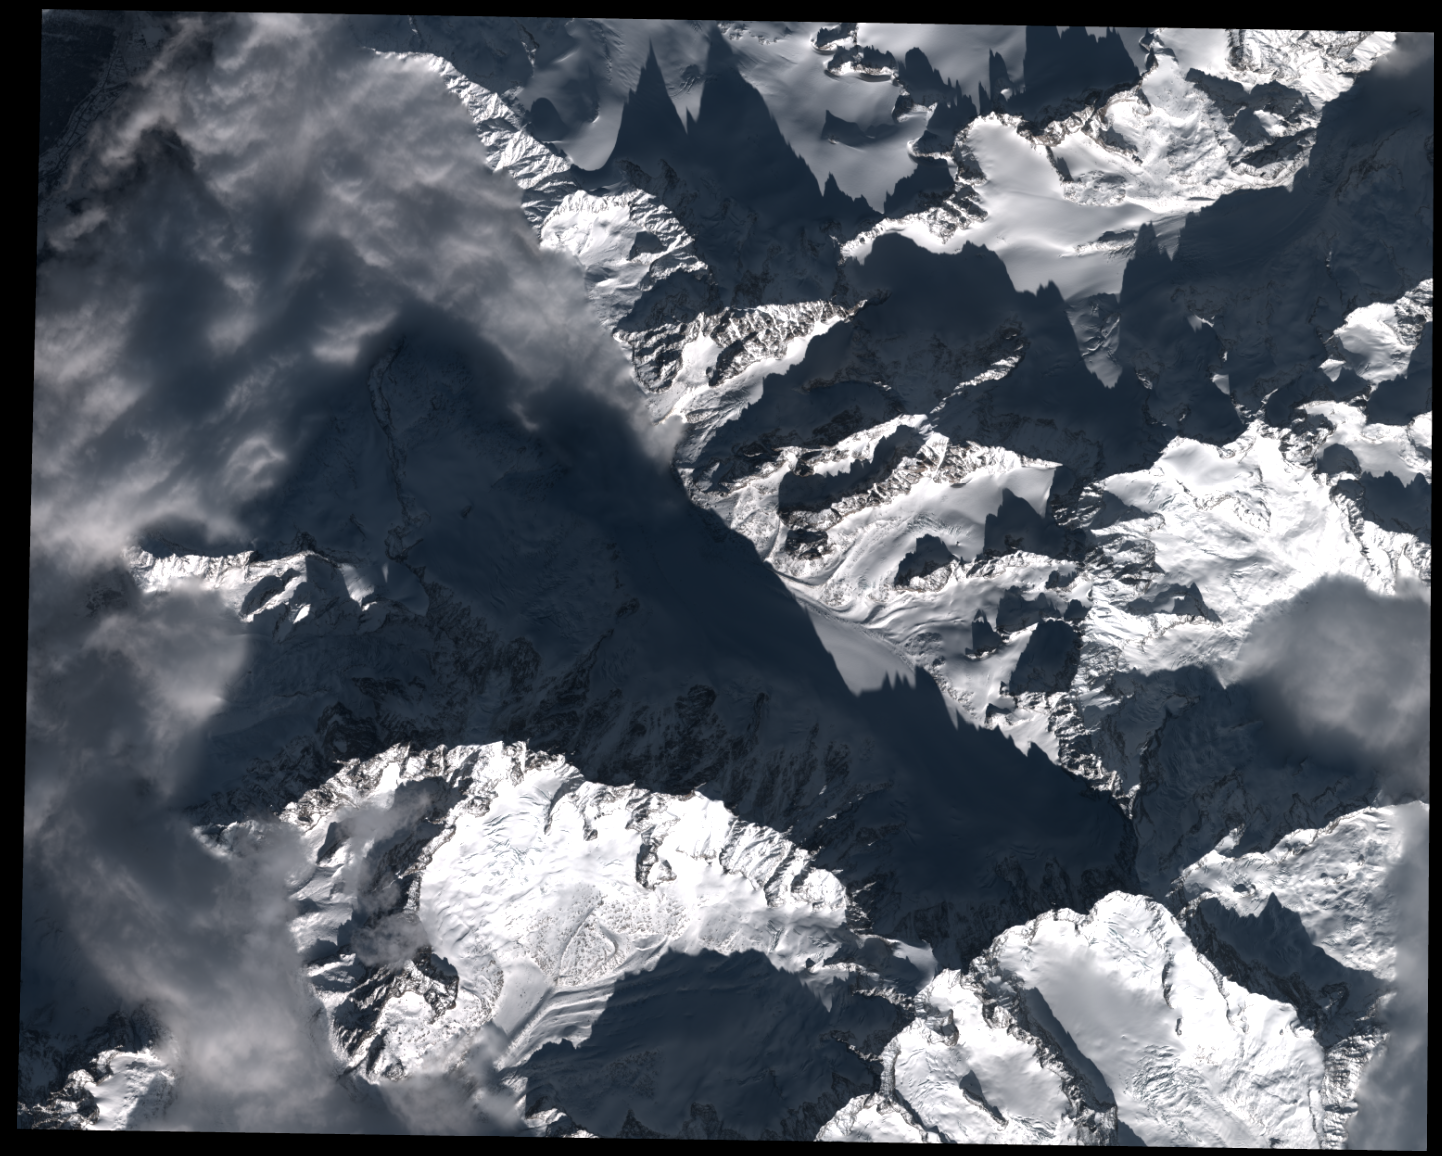
\includegraphics[keepaspectratio,width=1.005\paperwidth,height=1.1\paperheight]{images/argentiere_left.png}
\end{frame}

\vspace*{-6.5mm}
\begin{frame}[plain]
\hspace*{-11mm}
    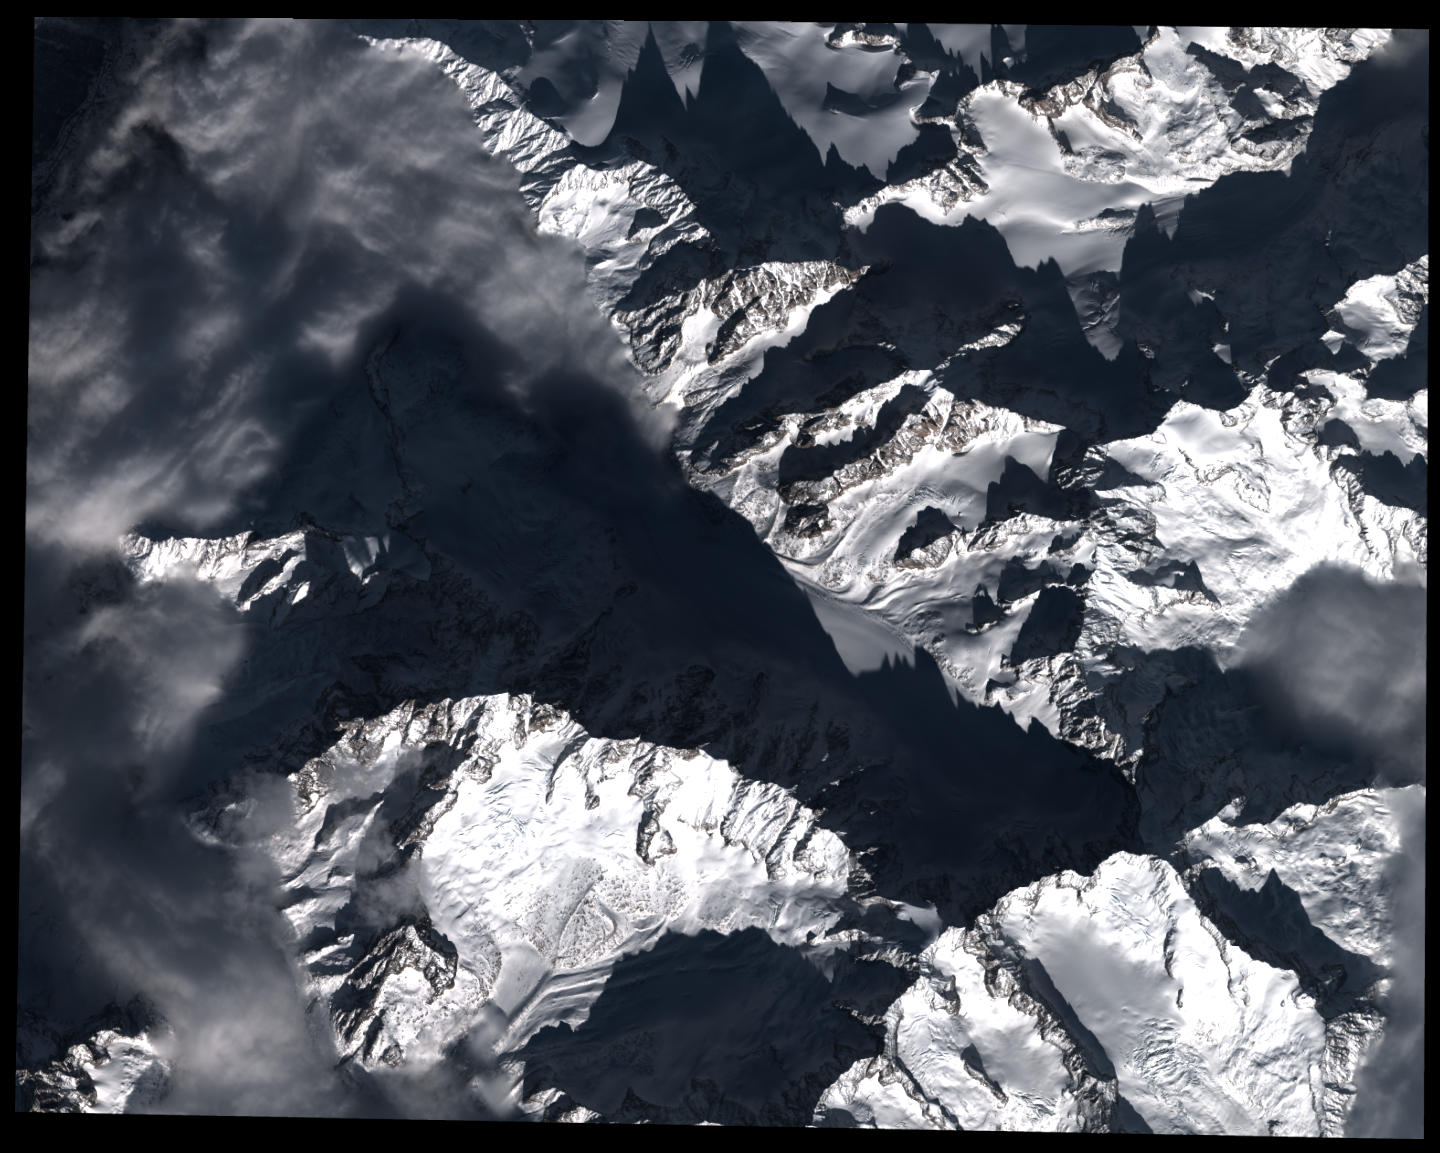
\includegraphics[keepaspectratio,width=1.005\paperwidth,height=1.1\paperheight]{images/argentiere_right.png}
\end{frame}

\vspace*{-6.5mm}
\begin{frame}[plain]
\hspace*{-11mm}
    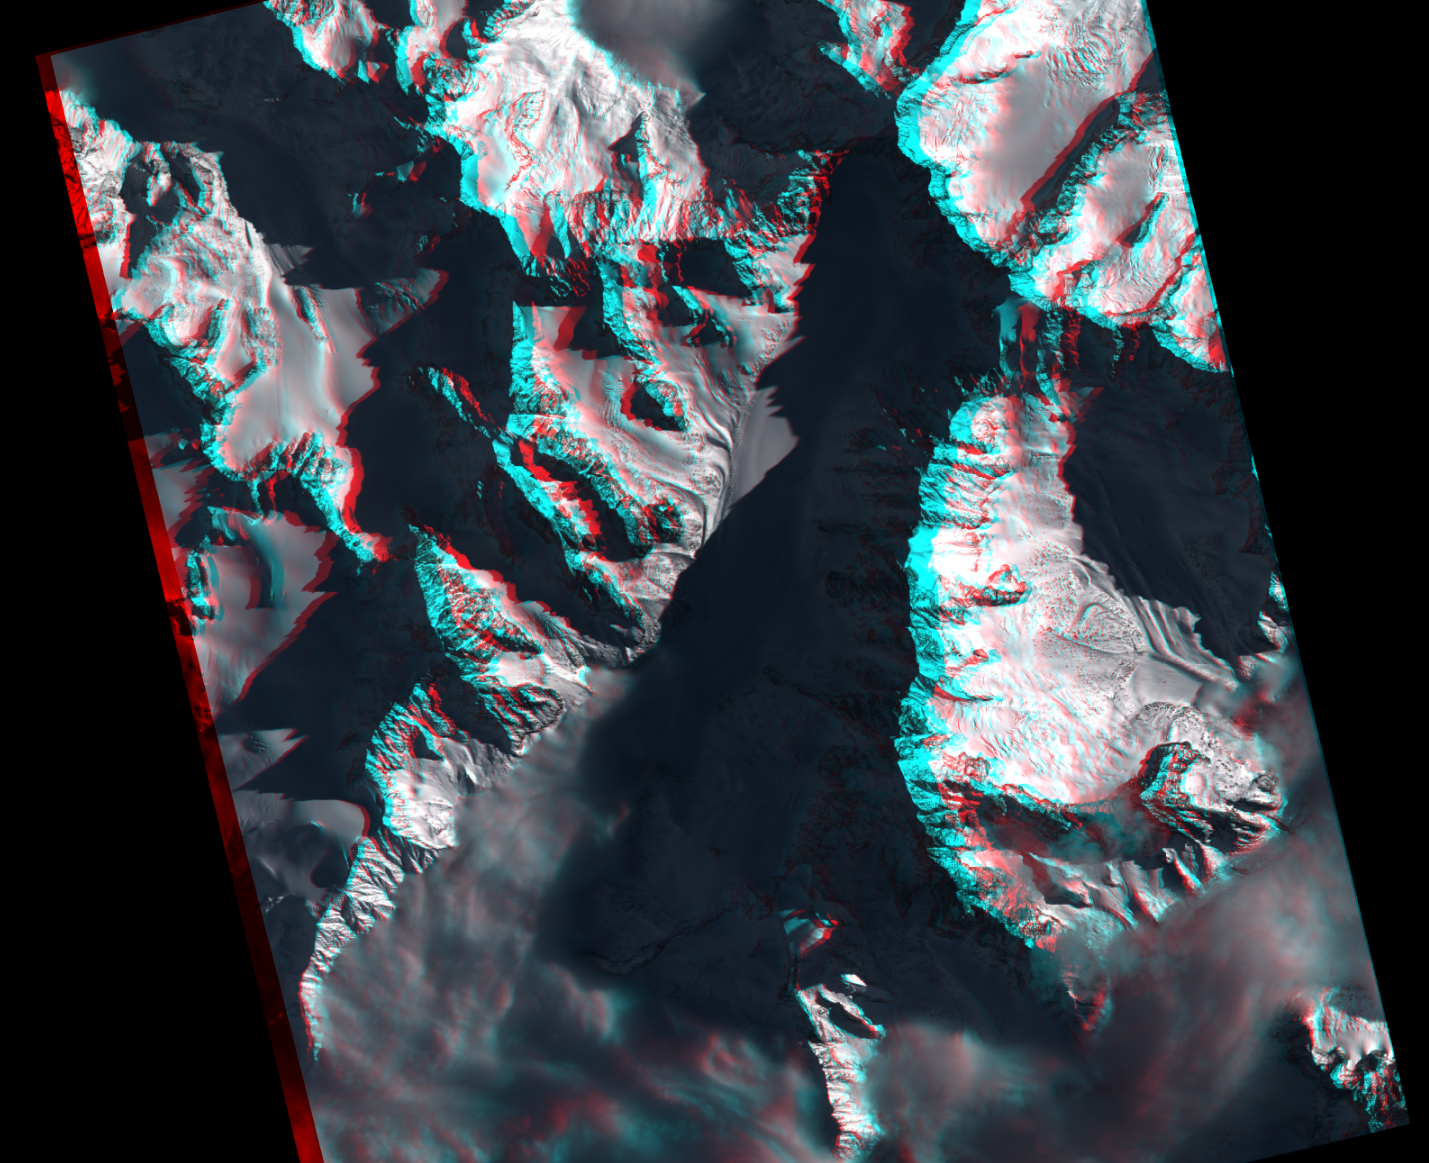
\includegraphics[keepaspectratio,width=1.005\paperwidth,height=1.1\paperheight]{images/argentiere_anaglyphe.png}
\end{frame}

\section{Caractéristiques clés}

\begin{frame}
\frametitle{Construite sur des logiciels libres tiers performants}
\begin{block}{Motivations}
\begin{itemize}
\item A chaque fois que c'est possible, l'Orfeo ToolBox s'appuie sur des
  logiciels libres tiers
\item Cette position d'intégrateur permet d'accroître rapidement le nombre de fonctions tout en assurant leurs validité
\item Elle permet également de créer de nouvelles fonctionnalités par hybridation
\end{itemize}
\end{block}

\begin{block}{Les logiciels tiers principaux}
\begin{itemize}
\item \href{www.itk.org}{ITK}: modélisation de la chaine de traitement
\item \href{www.gdal.org}{GDAL}: accès aux données images et vecteurs,
\item \href{www.ossim.org}{OSSIM}: modélisation géométrique des prises de vues,
\item \href{www.opencv.org}{OpenCV} et \href{www.libsvm.org}{LibSVM}: fonctionnalités de classification supervisée,
\item \href{www.muparser.org}{MuParser} et \href{www.muparserx.org}{MuParserX}:
analyse dynamique d'expressions mathématiques.
\end{itemize}
\end{block}


\end{frame}

\begin{frame}
\frametitle{Compatible (et disponible) pour un maximum de plateformes}
\begin{columns}
\column{0.5\textwidth}
\begin{block}{Objectif multi-plateforme}
\begin{itemize}
\item Compiler avec les versions récentes de:
\begin{itemize}
\item GCC
\item Clang
\item MinGW
\item Visual Studio\ldots
\end{itemize}
\item Des paquets binaires sont disponibles en fonction de la plateforme:
\begin{itemize}
\item Dépôt ubuntuGIS pour Ubuntu,
\item Intégration à OSGeo4W et paquets indépendants pour Windows,
\item Paquets MacPort, formule HomeBrew et image dmg pour Mac OS X\ldots
\end{itemize}
\end{itemize}
\end{block}
\column{0.5\textwidth}
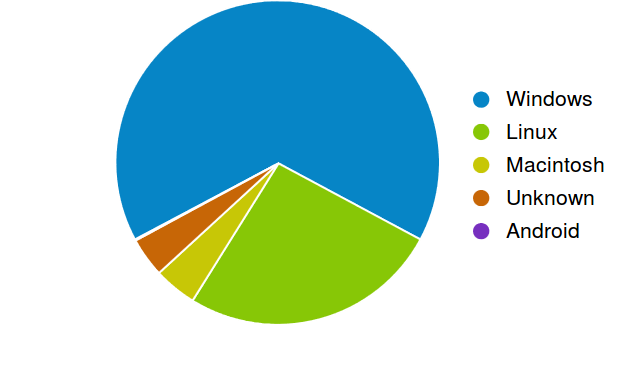
\includegraphics[width=\textwidth]{images/OTB4_download_sourceforge_os_crop.png}
\begin{center}
\tiny{Système d'exploitation des téléchargements sur Sourceforge (ne tient pas compte des autres dépôt)}
\end{center}
\end{columns}
\end{frame}

\begin{frame}
\frametitle{Flexibilité, passage à l'échelle: \textit{Pipeline}, \textit{Streaming} et \textit{multithreading}}

\begin{block}{Le modèle de \textit{Pipeline}}
\begin{center}
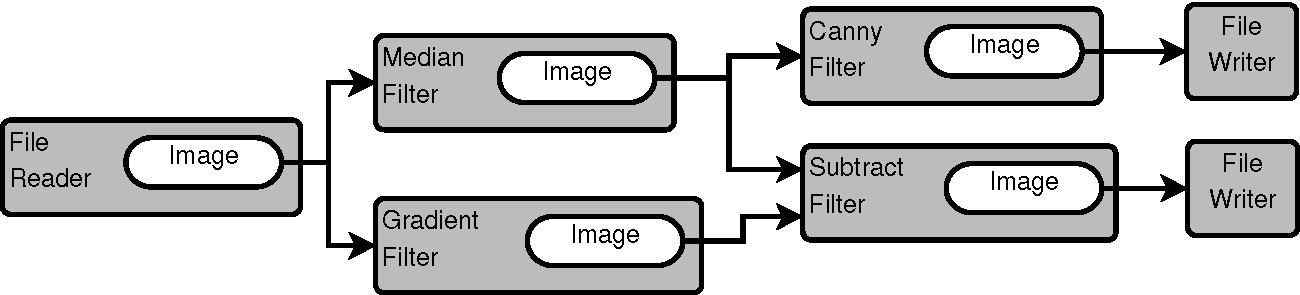
\includegraphics[width=0.7\textwidth]{images/ProcessObjectDataObject.png}
\end{center}
\end{block}
\vspace{-0.5cm}
\begin{block}{\textit{Streaming}}
\begin{center}
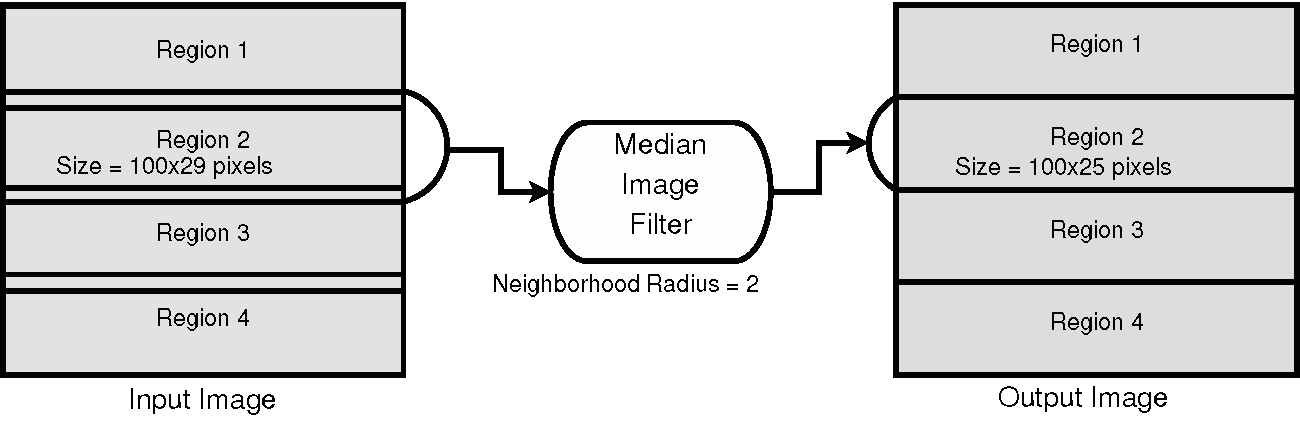
\includegraphics[width=0.7\textwidth]{images/StreamingImageDiagram.png}
\end{center}
\end{block}
\vspace{-0.5cm}
\begin{center}
\tiny{source: http://www.aosabook.org/en/itk.html}
\end{center}
\end{frame}

\begin{frame}
\frametitle{Flexibilité, passage à l'échelle: en coulisse ...}
\begin{center}
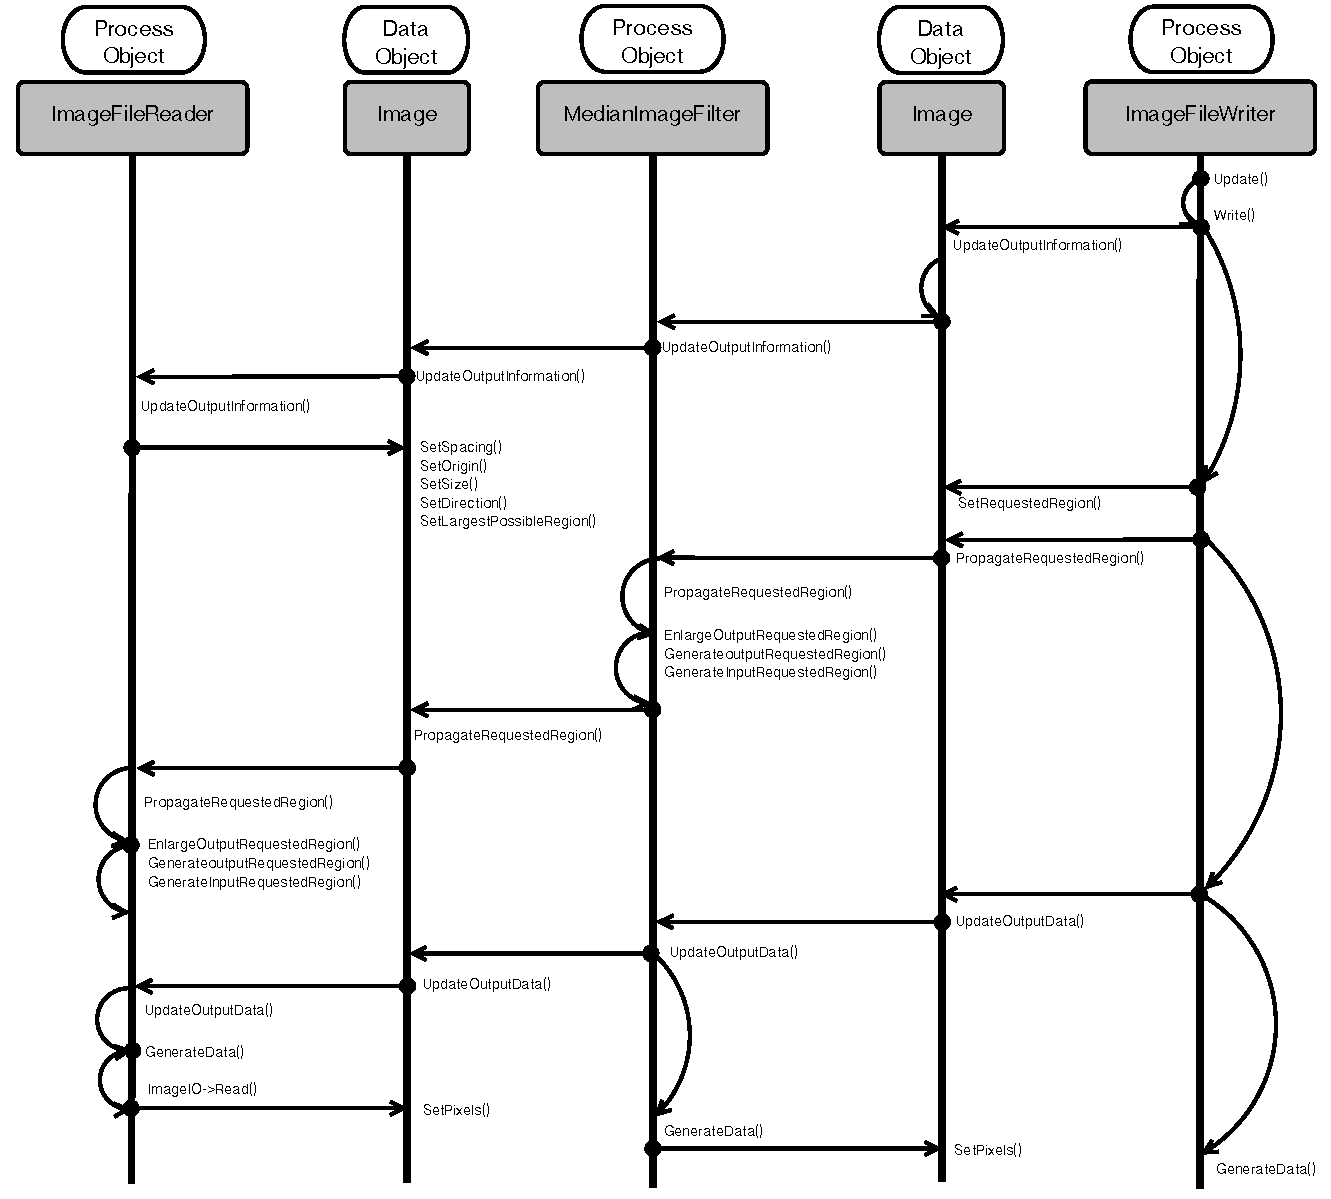
\includegraphics[width=0.6\textwidth]{images/ProcessObjectDataObjectInteractionUML.png}\\
\tiny{source: http://www.aosabook.org/en/itk.html}
\end{center}
\end{frame}

\begin{frame}
\frametitle{Proche de l'état de l'art}
\begin{itemize}
\item Veille technologique de l'équipe de développement
\item Implémentations d'algorithmes récents d'après publication. Ex.: profils morphologiques, segmentation MeanShift, textures de Haralick, points d'intérêt SURF \ldots
\item Implémentations de références contribuées par les auteurs de certains travaux en support à leur publication. Ex.: Large Scale MeanShift, fusion bayésienne, détection d'objets \ldots
\item Veille pour bénéficier des avancées des logiciels tiers. Ex.: algorithmes de \textit{machine learning} d'OpenCV,
\item Souvent: pour une même brique fonctionnelle, plusieurs algorithmes de complexités différentes disponibles sous une même interface.
\end{itemize}
\end{frame}


\begin{frame}
\frametitle{Un mot concernant le développement du logiciel}
\vspace{-0.5cm}
\begin{itemize}
\item Gestion de code source décentralisée: Git (migration depuis Mercurial en
  Juillet 2015)
\item C++ et suite CMake (CTest, CDash)
\item Développement guidé par les tests (TDD)
\item Gestion Agile (scrum)
\item Intégration continue et packaging automatisé
\end{itemize}
Tout les jours, environ 3000 tests sont compilés et rejoués sur 16
configurations différentes.
\begin{center}
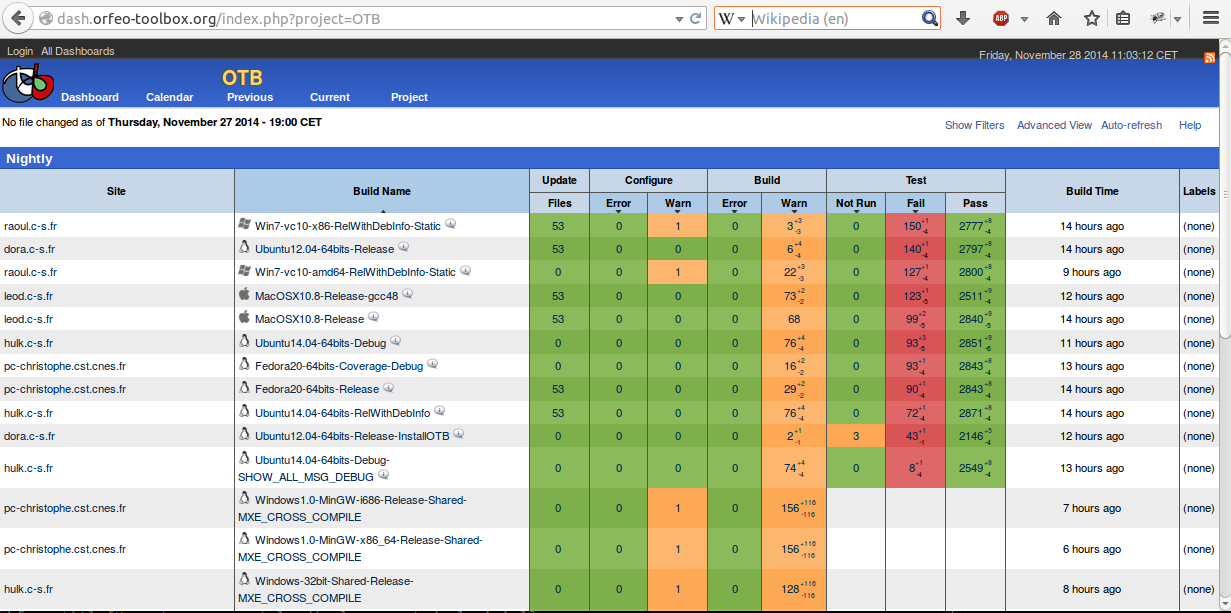
\includegraphics[width=\textwidth]{images/dashboard.png}
\end{center}
\end{frame}

\section{Comment utiliser OTB?}

\begin{frame}
\frametitle{Comment utiliser l'OTB?}
\vspace{-0.5cm}
\begin{center}
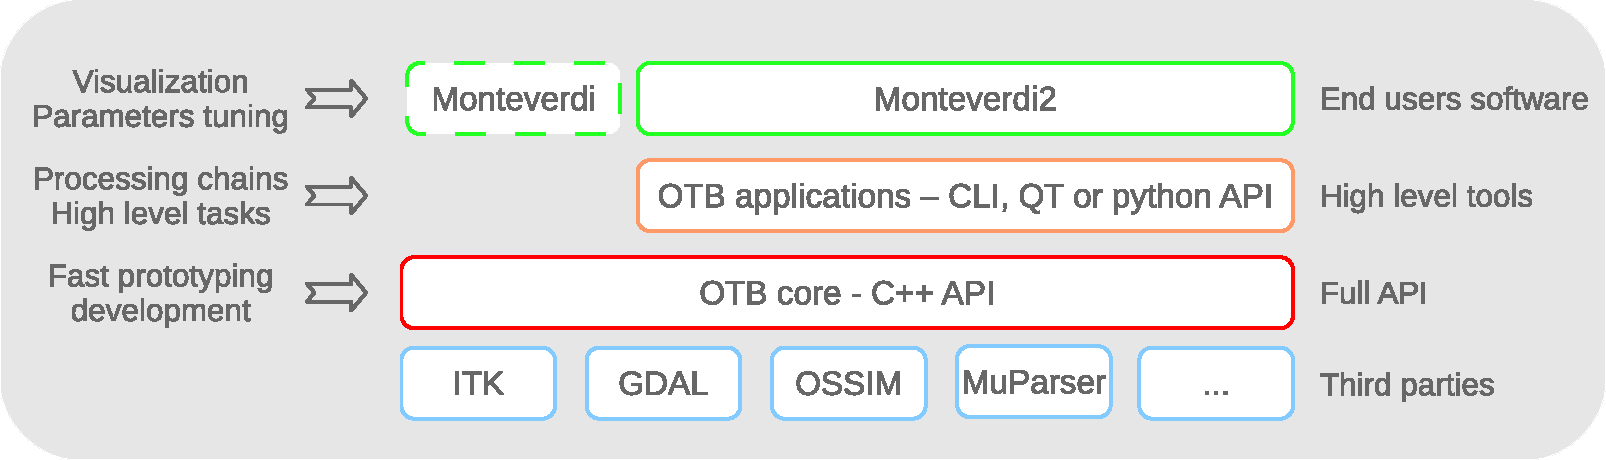
\includegraphics[width=\textwidth]{images/sandwich.pdf}
\end{center}
\vspace{-0.5cm}
\begin{block}{Écrire son propre code}
 Flexible, accès à l'API complète, demande une connaissance en C++
\end{block}
\begin{block}{Utiliser les applications}
 Fonctions de haut niveau (par ex. segmentation), appelable en ligne de commande, via une interface graphique, ou depuis Python. Peut être étendue (création d'applications)
\end{block}
\begin{block}{Utiliser Monteverdi}
Visualisation, gestion persistante des données, \textcolor{red}{Accès à l'ensemble des applications}
\end{block}
\end{frame}

\begin{frame}[fragile]
\frametitle{Show me the code!}
\begin{lstlisting}[language=c++,breaklines=true,breakatwhitespace=true,frame = tb,framerule = 0.25pt,fontadjust,backgroundcolor={\color{listlightgray}},basicstyle = {\ttfamily\tiny},keywordstyle = {\ttfamily\color{listkeyword}\textbf},identifierstyle = {\ttfamily},commentstyle = {\ttfamily\color{listcomment}\textit},stringstyle = {\ttfamily},showstringspaces = false,showtabs = false,numbers = none,numbersep = 2pt, numberstyle={\ttfamily\color{listnumbers}},tabsize = 2]
#include "otbImage.h"
#include "otbImageFileReader.h"
#include "otbImageFileWriter.h"
#include "itkCannyEdgeDetectionImageFilter.h"
#include "itkRescaleIntensityImageFilter.h"

int main(int argc, char * argv[])
{
  typedef double                      PixelType;
  typedef otb::Image<PixelType>       ImageType;

  typedef unsigned char               OutputPixelType;
  typedef otb::Image<OutputPixelType> OutputImageType;

  typedef otb::ImageFileReader<ImageType> ReaderType;
  ReaderType::Pointer reader = ReaderType::New();

  reader->SetFileName(argv[1]);

  typedef itk::CannyEdgeDetectionImageFilter
  <ImageType, ImageType> FilterType;
  FilterType::Pointer filter = FilterType::New();

  filter->SetInput(reader->GetOutput());

  typedef otb::ImageFileWriter<OutputImageType> WriterType;
  WriterType::Pointer writer = WriterType::New();

  writer->SetFileName(argv[2]);

  writer->SetInput(filter->GetOutput());

  writer->Update();
}
\end{lstlisting}
\end{frame}

\begin{frame}
\frametitle{Les applications: codées une fois, utilisables partout}
\begin{columns}
\column{0.5\textwidth}
\begin{itemize}
\item 87 applications sont livrées avec l'OTB
\item 1 application $=$ 1 librairie dynamique (plugin)
\item Les applications sont auto-descriptives et auto-documentées
\item Les applications peuvent etre étendues en dehors de l'OTB
\item Plusieurs interfaces sont disponibles pour utiliser les plugins:
\begin{itemize}
  \item Ligne de commande
  \item Interface Qt auto-générée
  \item Python
\end{itemize}
\item Les applications sont conçues pour une intégration facilitée dans des systèmes externes
\end{itemize}
\column{0.5\textwidth}
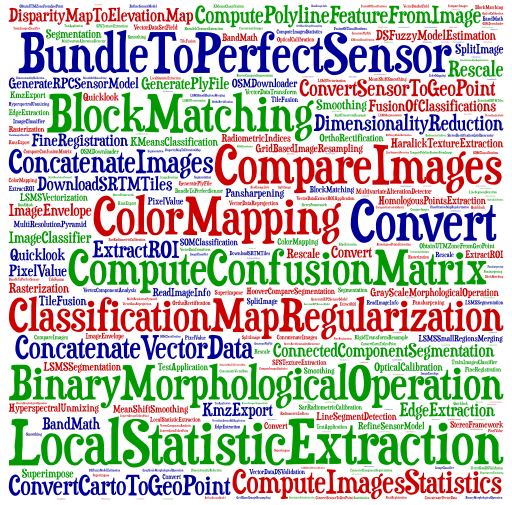
\includegraphics[width=\textwidth]{images/cloud_applications.png}
\end{columns}
\end{frame}



\begin{frame}[fragile]
\frametitle{Applications: appel depuis la ligne de commande}
\begin{scriptsize}
\vspace{-0.5cm}\begin{verbatim}
$ otbcli_OrthoRectification

ERROR: Waiting for at least one parameter...
This is the OrthoRectification application, version 5.2.1
This application allows to ortho-rectify optical images from supported sensors.

Complete documentation: http://www.orfeo-toolbox.org/Applications/OrthoRectification.html

Parameters:
        -progress                <boolean>        Report progress
MISSING -io.in                   <string>         Input Image  (mandatory)
MISSING -io.out                  <string> [pixel] Output Image  [pixel=uint8/uint16/int16/uint32/int32/float/double] (default value is float) (mandatory)
        -map                     <string>         Output Cartographic Map Projection [utm/lambert2/lambert93/wgs/epsg] (mandatory, default value is utm)
        -map.utm.zone            <int32>          Zone number  (mandatory, default value is 31)
        -map.utm.northhem        <boolean>        Northern Hemisphere  (optional, off by default)
        -map.epsg.code           <int32>          EPSG Code  (mandatory, default value is 4326)
        -outputs.mode            <string>         Parameters estimation modes [auto/autosize/autospacing/outputroi/orthofit] (mandatory, default value is auto)
MISSING -outputs.ulx             <float>          Upper Left X  (mandatory)
MISSING -outputs.uly             <float>          Upper Left Y  (mandatory)
MISSING -outputs.sizex           <int32>          Size X  (mandatory)
MISSING -outputs.sizey           <int32>          Size Y  (mandatory)
MISSING -outputs.spacingx        <float>          Pixel Size X  (mandatory)
MISSING -outputs.spacingy        <float>          Pixel Size Y  (mandatory)
        -outputs.lrx             <float>          Lower right X  (optional, off by default)
        -outputs.lry             <float>          Lower right Y  (optional, off by default)
        -outputs.ortho           <string>         Model ortho-image  (optional, off by default)
        -outputs.isotropic       <boolean>        Force isotropic spacing by default  (optional, on by default)
        -outputs.default         <float>          Default pixel value  (optional, on by default, default value is 0)
        -elev.dem                <string>         DEM directory  (optional, off by default)
        -elev.geoid              <string>         Geoid File  (optional, off by default)
        -elev.default            <float>          Default elevation  (mandatory, default value is 0)
        -interpolator            <string>         Interpolation [bco/nn/linear] (mandatory, default value is bco)
\end{verbatim}
\end{scriptsize}
\end{frame}

\begin{frame}[fragile]
\frametitle{Applications OTB: Interface graphique}
\begin{center}
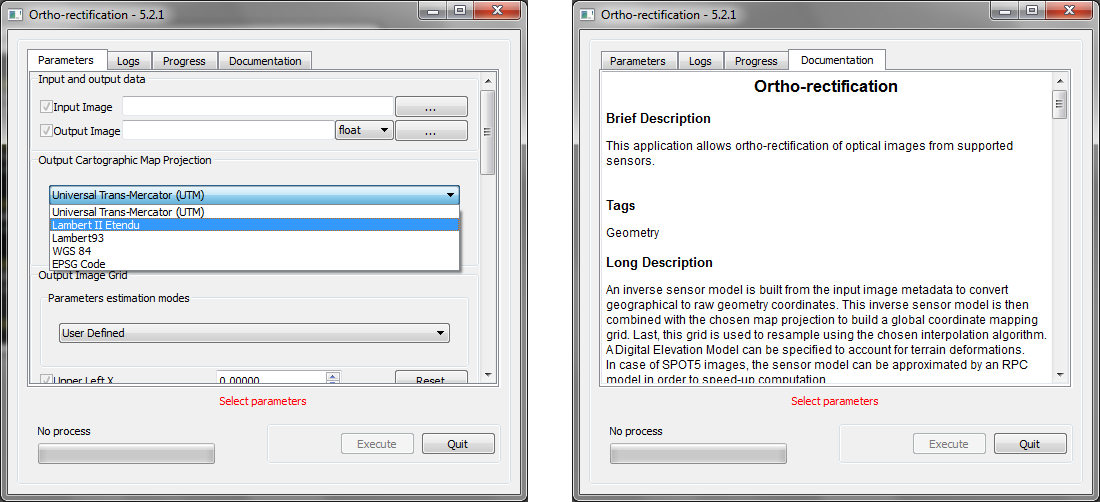
\includegraphics[width=1\textwidth]{images/otbgui.png}
\end{center}
\end{frame}

\begin{frame}[fragile]
\frametitle{Applications: appel depuis l'interface Python}
\begin{lstlisting}[language=python,breaklines=true,breakatwhitespace=true,frame = tb,framerule = 0.25pt,fontadjust,backgroundcolor={\color{listlightgray}},basicstyle = {\ttfamily\tiny},keywordstyle = {\ttfamily\color{listkeyword}\textbf},identifierstyle = {\ttfamily},commentstyle = {\ttfamily\color{listcomment}\textit},stringstyle = {\ttfamily},showstringspaces = false,showtabs = false,numbers = none,numbersep = 6pt, numberstyle={\ttfamily\color{listnumbers}},tabsize = 2]
#!/usr/bin/python

# Import the otb applications package
import otbApplication

# The following line creates an instance of the OrthoRectification application
OrthoRectification = otb.Registry.CreateApplication("OrthoRectification")

# The following lines set all the application parameters:
OrthoRectification.IO.IN = "QB_TOULOUSE_MUL_Extract_500_500.tif"
OrthoRectification.IO.OUT = "QB_Toulouse_ortho.tif"

app.MAP = 'epsg'
app.MAP.EPSG.CODE = 32768

# The following line execute the application
OrthoRectification.ExecuteAndWriteOutput()
\end{lstlisting}
\end{frame}


\begin{frame}
\frametitle{Monteverdi (accès aux applications OTB)}
\begin{minipage}[t][6cm][t]{\textwidth}
\begin{center}
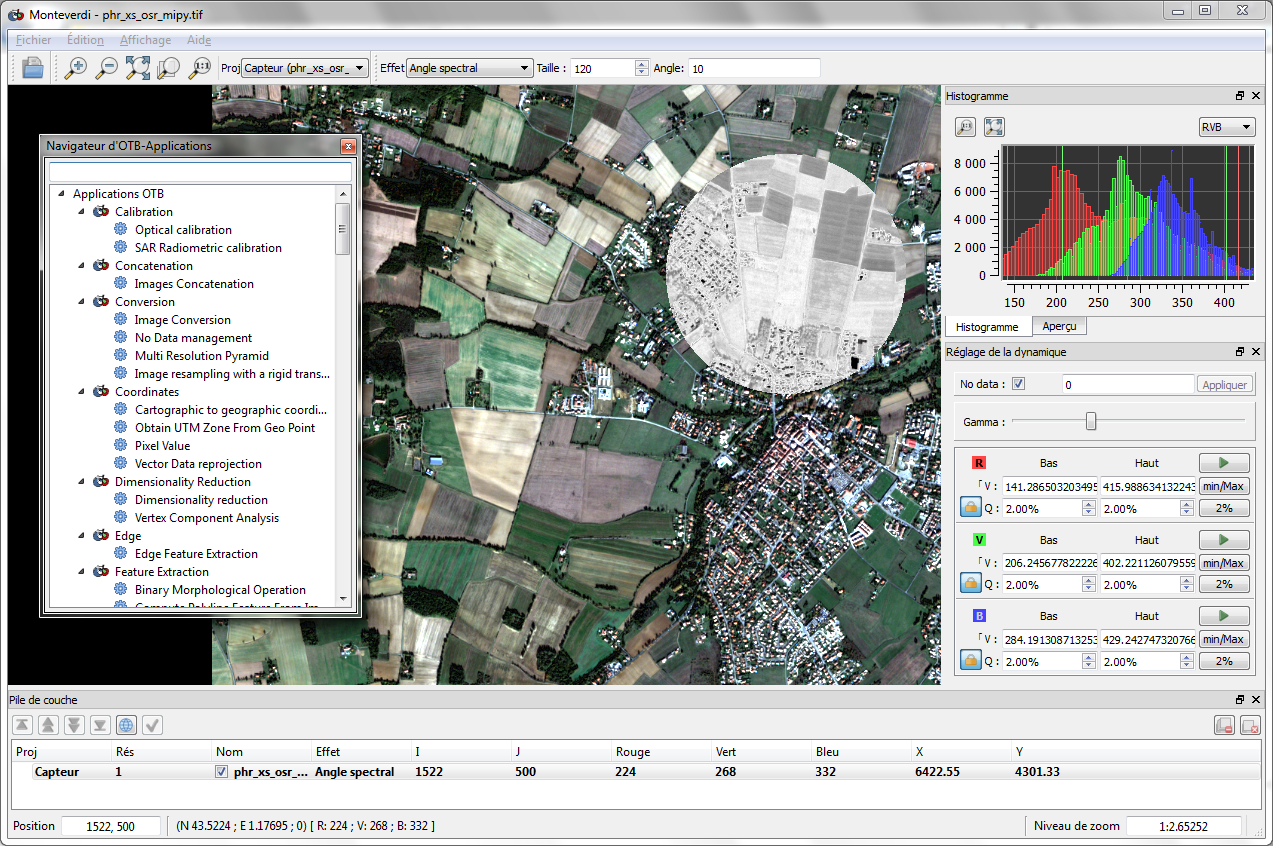
\includegraphics[width=1.0\textwidth]{images/monteverdi.png}
\end{center}
\end{minipage}
\end{frame}

%\vspace*{-3.0mm}
\begin{frame}
  \frametitle{QGIS (accès aux applications OTB)}
\begin{minipage}[t][6cm][t]{\textwidth}
\begin{center}
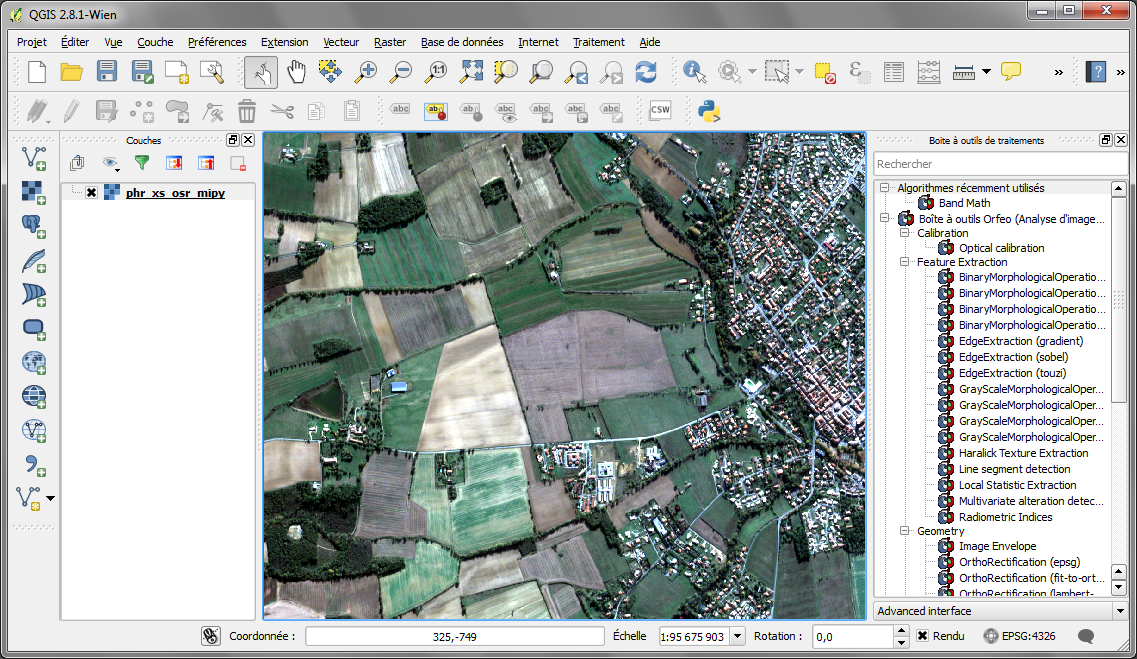
\includegraphics[width=1\textwidth]{images/otb_in_qgis.png}
\end{center}
\end{minipage}
\end{frame}


\section{Quoi de neuf dans l'OTB?}

\begin{frame}
\frametitle{Modularité (inspirée de l'organisation du code ITK 4.x)}
\begin{block}{Qu'est ce qui change?}
\begin{itemize}
\item Une meilleure organisation du code, en modules cohérents:
  \begin{itemize}
    \item OTB 4.4.0: 1672 fichiers dans 26 répertoires
    \item OTB 5.0: 1627 fichiers dans 124 modules répartis en 16 groupes
  \end{itemize}
\item Les modules sont complets: tests, code source, applications sont regroupés
\item Chaque module peut etre activé ou non, avec gestion des dépendances
\item Ca fonctionne! Plusieurs contributions \url{https://www.orfeo-toolbox.org/external-projects/}

\end{itemize}
\end{block}

\begin{block}{Quels sont les avantages?}
\begin{itemize}
\item Les logiciels tiers sont importés dans des modules désactivables comme les autres
\item Beaucoup de magie CMake (moins de code cmake, plus de choses automatisées)
\item La documentation doxygen reflète l'organisation en groupes/modules
\item Les contributions sont facilitées, notamment avec le mécanisme de
  \textit{remote module}
\item ça fonctionne! Déjà beaucoup de modules externes contribués: \url{https://www.orfeo-toolbox.org/external-projects/}
\end{itemize}
\end{block}
\end{frame}

\begin{frame}
\frametitle{Contribuer son module OTB}
\begin{block}{Schéma ITK}
\begin{center}
 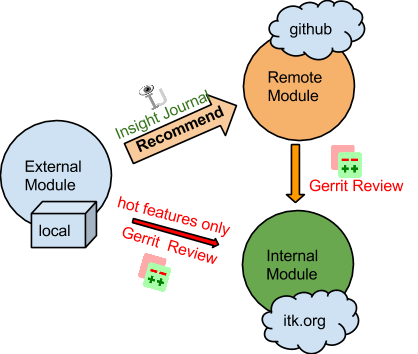
\includegraphics[width=0.4\textwidth]{images/itk-remote-module.png}
\end{center}
\end{block}
\end{frame}


\begin{frame}
\frametitle{Superbuild}
\begin{block}{Avant OTB 4.4.0}
\begin{itemize}
\item Certaines dépendances (mais pas toutes) peuvent etre compilée en interne
\item Leur code source est intégré à celui de l'Orfeo ToolBox (pas une bonne pratique en général)
\end{itemize}
\end{block}

\begin{block}{Dans OTB 5.0, on Superbuild!}
\begin{itemize}
\item Il n'y a plus de logiciels tiers dans l'OTB
\item Il existe un projet séparé appelé Superbuild, qui télécharge, configure, compile et installe chaque dépendance dans sa bonne version
\item On peut ainsi compiler une OTB complète avec très peu de pré-requis (cmake, gcc, zlib, curl), et totalement automatiquement
\item Il existe également un mode \textit{offline} pour compiler l'OTB en avion (ou toute autre situation sans accès internet)
\end{itemize}
\end{block}
\end{frame}

\begin{frame}
\frametitle{Project Steering Committee}
\begin{itemize}
\item Le PSC est un système de gouvernance ouverte
\item Il s'agit d'une entité de coordination plus qu'un organisme de décision
\item Animation de la communauté, et grandes orientations du projet
\item Tout le monde peut en devenir membre (nouveau membre = vote)
\item Les décisions et les débats sont publics (sur la liste de diffusion pour les développeurs)
\item Les statuts sont publics\footnote{\url{http://wiki.orfeo-toolbox.org/index.php/Project_Steering_Committee}}
\end{itemize}
\end{frame}

\begin{frame}
\frametitle{Quoi de neuf dans l'OTB 5.2?}
\begin{block}{Quoi de neuf dans la version 5.2 (Déc 2015)?}
\begin{itemize}
\item Nouvelles applications pour le traitement SAR (polarimétrie)
\item Support des produits Sentinel-1
\item Calibration radiométrique image SAR (Sentinel1 et Radarsat2)
\item Méthodes pour le filtrage du Speckle (Frost, Lee, GammaMAP, Kuan)
\item Mode régression et carte de confiance pour la classification
\item Amélioration accès OTB en Python
\item Compatibilité avec Gdal 2.0 et support des images Sentinel-2
\end{itemize}
\end{block}

\begin{block}{Goodbye Monteverdi2, welcome Monteverdi 3.0}
\begin{itemize}
\item Léger et performant
\item Affichage mosaique d'images ou série multi-temporelle
\item Outils de visualisation performants(contraste local, gradient\ldots)
\item Accès aux applications OTB
\end{itemize}
\end{block}
\end{frame}

\section{Conclusion et perspectives}
\begin{frame}
\frametitle{Combien d'utilisateurs ?}
\begin{columns}[c]
\column{0.5\textwidth}
\begin{block}{Difficile à dire \ldots}
\begin{itemize}
    \item $\approx$ 600 membres sur la liste utilisateurs
    \item $\approx$ Entre 100 et 150 messages par mois
    \item $\approx$ 100 membres sur la liste développeurs
    \item $\approx$ 118 comptes sur le système de gestion des bugs
    \item $\approx$ 50 contributeurs (listé dans la documentation)
    \item $\approx$ 3400 téléchargements for OTB 5.0
  \end{itemize}
\end{block}
\column{0.5\textwidth}
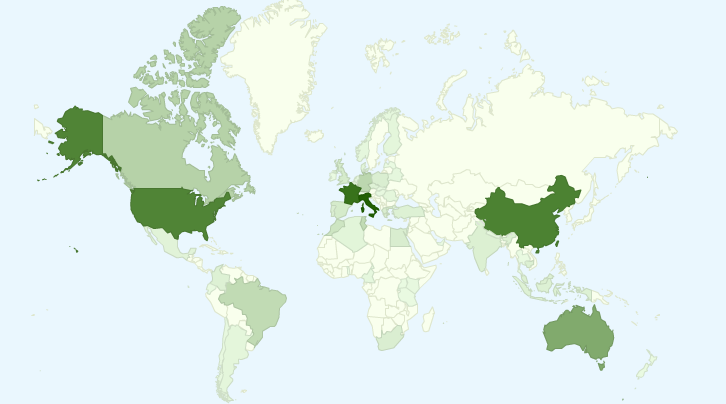
\includegraphics[width=\textwidth]{images/OTB4_download_sourceforge_country_crop.png}
\end{columns}
\end{frame}

\begin{frame}
\frametitle{Les réussites de l'OTB}
\vspace{-0.5cm}
\begin{columns}
\column{0.6\textwidth}
\begin{itemize}
\item l'OTB a été utile à (certains) des utilisateurs ORFEO!
\item L'OTB a traité avec succès plus de 619 images Pléiades pour le site web RTU,
\item L'OTB fournit beaucoup de fonctions utiles pour la télédétection dans un \textbf{unique outil}
\item L'OTB est (a été) l'unique logiciel open-source compatible avec les images Pléiades (grâce à OpenJPEG)
\item L'OTB égale ou dépasse les outils de l'état de l'art (libre et commercial) pour certaines fonctions:
\begin{itemize}
\item La calculatrice de bandes,
\item La segmentation de scène complètes,
\item La classification à l'échelle d'une scène complète avec un grand choix d'algorithmes,
\item Les ponts entre la télédétection et le systèmes d'information géographique\ldots
\end{itemize}
\item Au delà d'ORFEO, l'OTB est déjà utilisée dans plusieurs projets et logiciels
\end{itemize}
\column{0.4\textwidth}
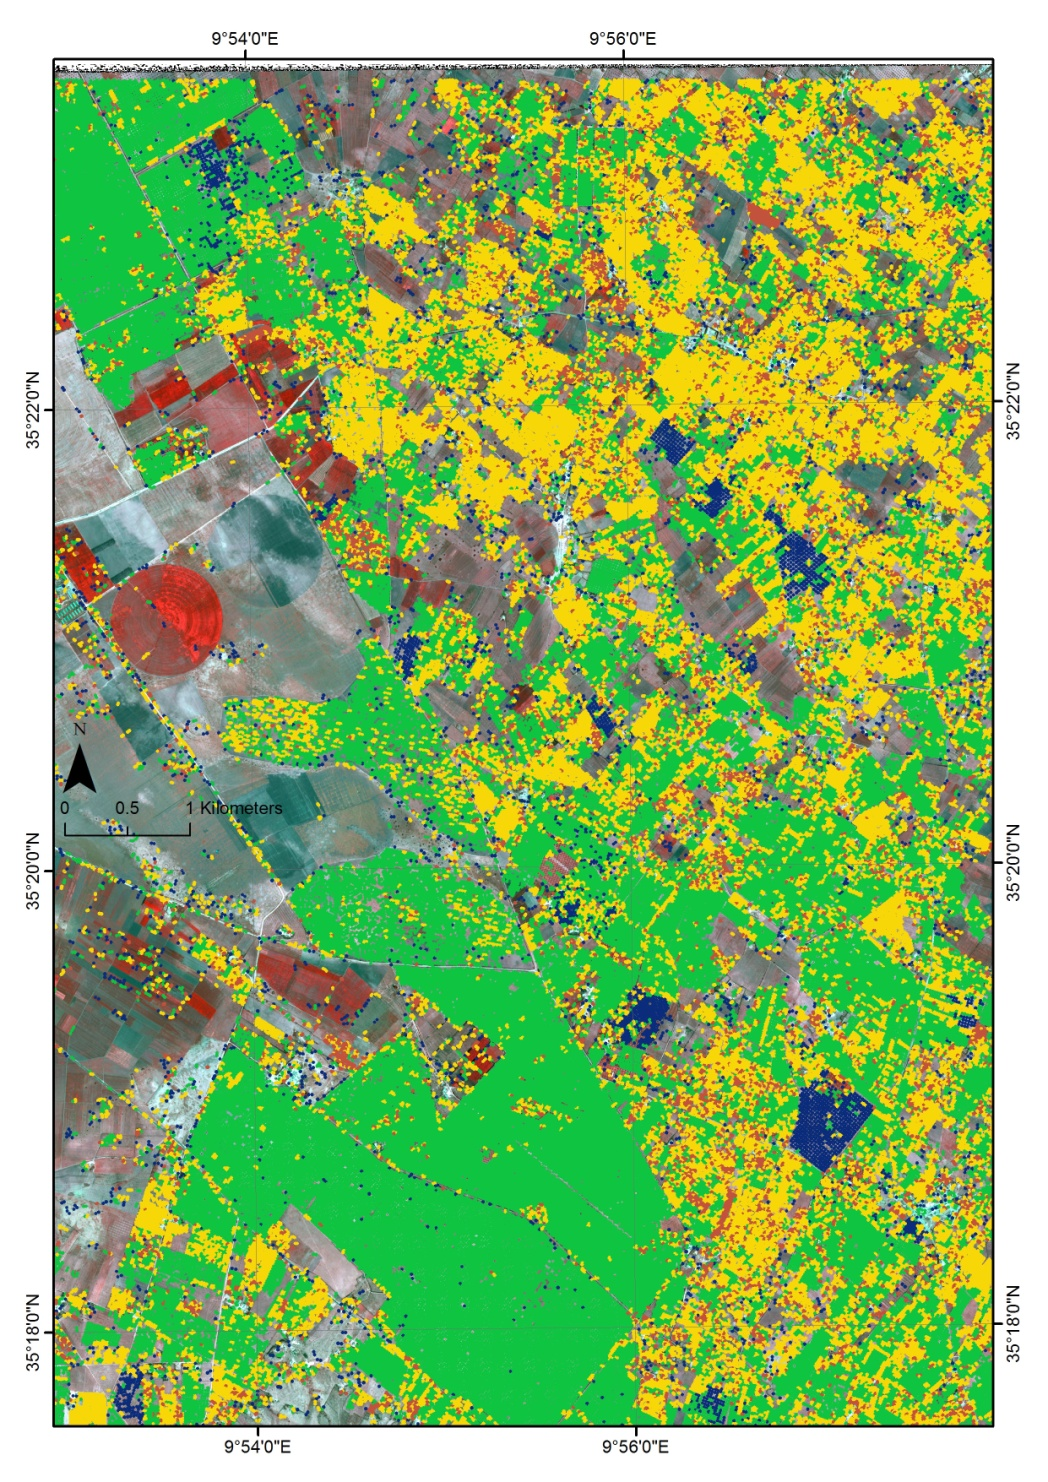
\includegraphics[width=0.9\textwidth]{images/resultats_ird.png}\\
\tiny{Carte thématique à partir d'une segmentation par l'OTB, B. Mougenot~-~IRD}
\end{columns}
\end{frame}

\begin{frame}
\frametitle{Projets et logiciels utilisant l'OTB}
\begin{columns}
  \column{0.5\textwidth}
  \begin{itemize}
    \item Les applications OTB applications sont disponibles dans le module de traitement de QGIS
    \item L'OTB est utilisée dans certains composant des segments sols S2 et
      Venus (CNES et ESA)
    \item Logiciel educatif Terr'Image
    \item Utiliser pour générer des produits à l'échelle nationale en France
      dans THEIA
    \item Projet EA S2 Agriculture
    \item Le logiciel Gnorasi (National Technical University of Athens)
    \item Le projet Vahine (traitement d'images hyperspectrales pour l'astrophysique), IPAG
    \item Projet GEOSUD (IRSTEA)
    \item Le programme de recherche TCM (ETS Quebec)
  \end{itemize}
  \column{0.65\textwidth}
\begin{center}
  \includegraphics[width=0.6\textwidth,height=0.35\textheight]{images/Carte_17Classes.png}\\
  \tiny{Produit occupation du sol THEIA (CESBIO)}
  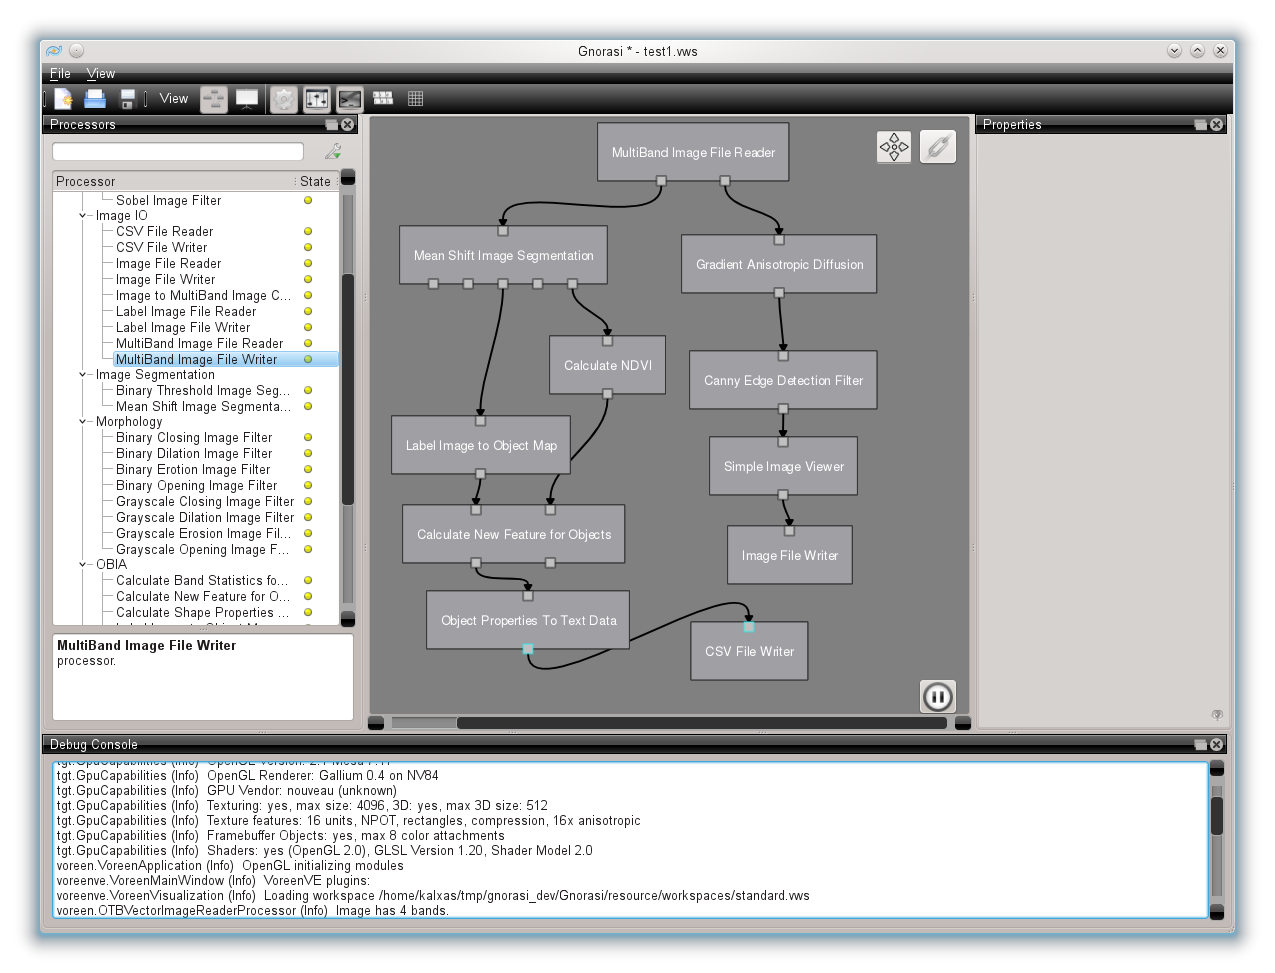
\includegraphics[width=\textwidth]{images/gnorasi2.png}\\
  \tiny{Le logiciel Gnorasi}
\end{center}
\end{columns}
\end{frame}

\begin{frame}
\frametitle{Un système complexe: chaos et effets de bord}
\begin{center}
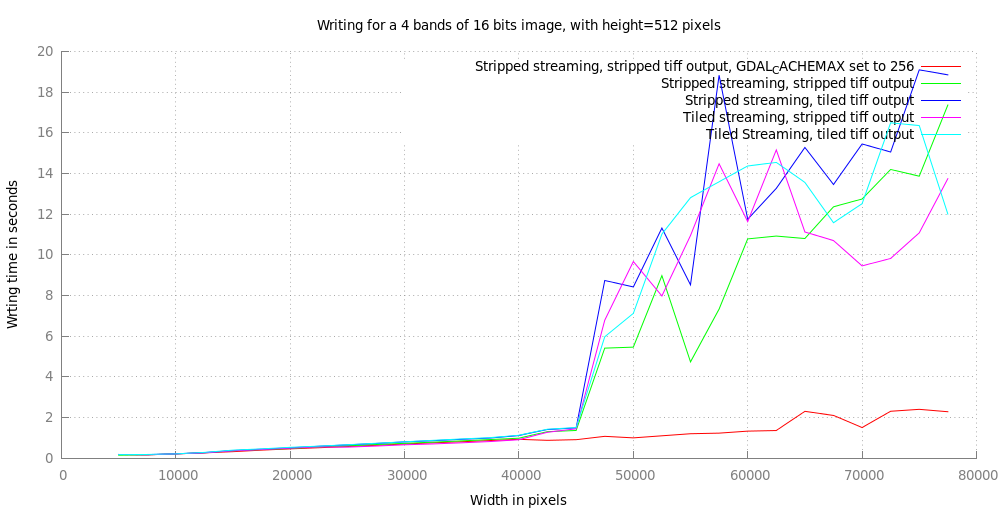
\includegraphics[width=\textwidth]{images/Writing.png}\\
\tiny{Effets des paramètres d'encodage tif et du streaming sur les performances d'une chaîne de traitement}
\end{center}
\end{frame}

\begin{frame}
\frametitle{Support/Aide/Contribution}
\vspace{-0.2cm}
\begin{block}{Ressources}
\vspace{-0.2cm}
\begin{description}
\item[Site web] \href{http://www.orfeo-toolbox.org}{orfeo-toolbox.org}
\item[Wiki] \href{http://wiki.orfeo-toolbox.org}{wiki.orfeo-toolbox.org}
\item[Blog] \href{http://blog.orfeo-toolbox.org}{blog.orfeo-toolbox.org}
\end{description}
\end{block}
\vspace{-0.2cm}
\begin{block}{Documentation et aide}
\vspace{-0.2cm}
\begin{description}
\item[Doxygen] \href{http://www.orfeo-toolbox.org/doxygen/}{doxygen}
\item[Documentation] Software Guide et CookBook (remote sensing recipes)
\item[Liste de diffusion utilisateurs] otb-users@googlegroups.com
\item[Liste de diffusion développeurs] otb-developers@googlegroups.com
\end{description}
\end{block}
\vspace{-0.2cm}
\begin{block}{Follow-up}
\vspace{-0.2cm}
\begin{description}
\item[Où se trouve le code?] \href{http://git.orfeo-toolbox.org}{git.orfeo-toolbox.org}
\item[Vous avez trouvé un bug?] \href{http://bugs.orfeo-toolbox.org}{bugs.orfeo-toolbox.org}
\item[Agile?] \href{http://scrum.orfeo-toolbox.org}{scrum.orfeo-toolbox.org}
\item[Météo?] \href{http://dash.orfeo-toolbox.org}{dash.orfeo-toolbox.org}
\end{description}
\end{block}
\end{frame}

\begin{frame}
\frametitle{Merci pour votre attention. Des questions?}
\begin{minipage}[t][6cm][t]{\textwidth}
\begin{center}
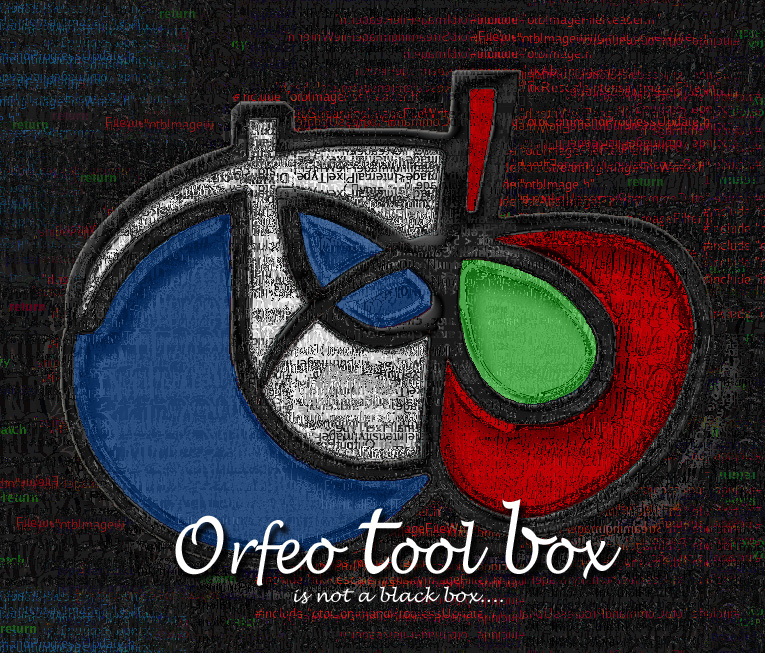
\includegraphics[width=0.65\textwidth]{images/LOGOTB_blackbox.png}
\end{center}
\end{minipage}
\end{frame}

\end{document}
